\documentclass{article}
\newcommand{\ImageWidth}{11cm}
\usepackage{tikz}
\usetikzlibrary{decorations.pathreplacing,positioning, arrows.meta}

\usepackage{amsmath} % for \text
\tikzset{>=latex} % for LaTeX arrow head
\usepackage{xcolor}
\colorlet{myblue}{black!40!blue}
\colorlet{myred}{black!40!red}

\usepackage{dcolumn}

\begin{document}         
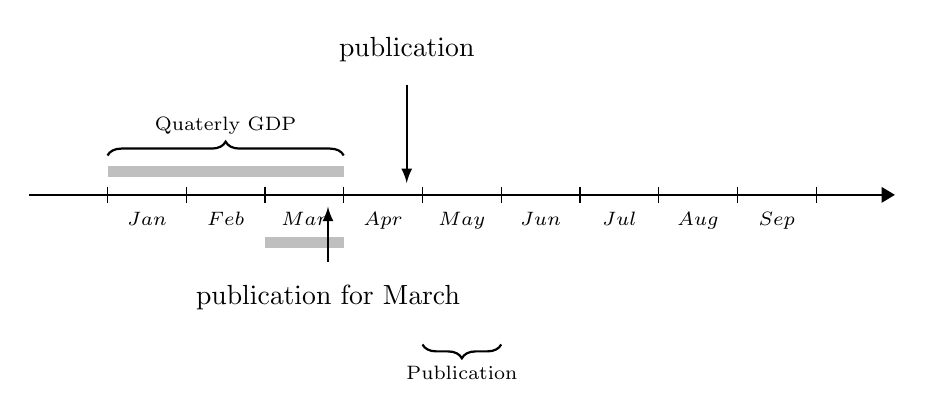
\begin{tikzpicture}
% draw horizontal line   
\draw[thick, -Triangle] (0,0) -- (\ImageWidth,0) node[font=\scriptsize,below left=3pt and -8pt]{ };

% draw vertical lines
\foreach \x in {1,...,10}
\draw (\x cm,3pt) -- (\x cm,-3pt);

\foreach \x/\descr in {1.5/Jan, 2.5/Feb, 3.5/Mar, 4.5/Apr, 5.5/May, 6.5/Jun, 7.5/Jul, 8.5/Aug,9.5/Sep}
\node[font=\scriptsize, text height=1.75ex,
text depth=.5ex] at (\x,-.3) {$\descr$};

% colored bar up
\foreach \x/\perccol in
{1/100,2/75,3/25}
\draw[lightgray, line width=4pt] 
(\x,.3) -- +(1,0);

% colored bar down
\foreach \x/\perccol in
{3/25}
\draw[lightgray, line width=4pt] 
(\x,-.6) -- +(1,0);


% braces
\draw [thick ,decorate,decoration={brace,amplitude=5pt}] (1,0.5)  -- +(3,0) 
       node [black,midway,above=4pt, font=\scriptsize] {Quaterly GDP};
\draw [thick,decorate,decoration={brace,amplitude=5pt}] (6,-1.9) -- +(-1,0)
      node [black,midway,font=\scriptsize, below=4pt] {Publication};

% time of publication
\node[align=center] at (4.8,1.85) {publication};
\draw [thick,->] (4.8,1.4) -- (4.8,0.15);
\node[align=center] at (3.8,-1.3) {publication for March};
\draw [thick,->] (3.8,-0.85) -- (3.8,-0.15);
\end{tikzpicture}


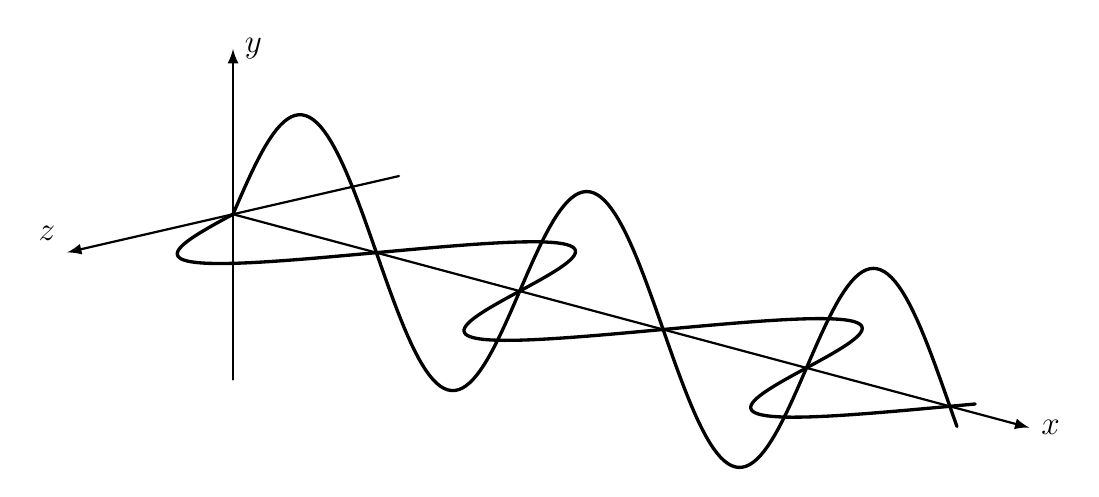
\begin{tikzpicture}[x=(-15:1.2), y=(90:1.0), z=(-150:1.0),
                    line cap=round, line join=round,
                    axis/.style={black, thick,->},
                    vector/.style={>=stealth,->}]
  \large
  \def\A{1.5}
  \def\nNodes{5} % use even number
  \def\nVectorsPerNode{8}
  \def\N{\nNodes*40}
  \def\xmax{\nNodes*pi/2*1.01}
  \pgfmathsetmacro\nVectors{(\nVectorsPerNode+1)*\nNodes}
 
  \def\vE{\mathbf{E}}
  \def\vB{\mathbf{B}}
  \def\vk{\mathbf{\hat{k}}}
 
  \draw[very thick,variable=\t,domain=0:\nNodes*pi/2*1.01,samples=\N]
    plot (\t,{\A*sin(\t*360/pi)},0);
  \draw[very thick,variable=\t,domain=0:\nNodes*pi/2*1.01,samples=\N]
    plot (\t,0,{\A*sin(\t*360/pi)});
 
  % main axes
  \draw[axis] (0,0,0) -- ++(\xmax*1.1,0,0) node[right] {$x$};
  \draw[axis] (0,-\A*1.4,0) -- (0,\A*1.4,0) node[right] {$y$};
  \draw[axis] (0,0,-\A*1.4) -- (0,0,\A*1.4) node[above left] {$z$};
 
  % ...
 
\end{tikzpicture}



% Electromagnetic wave - colored
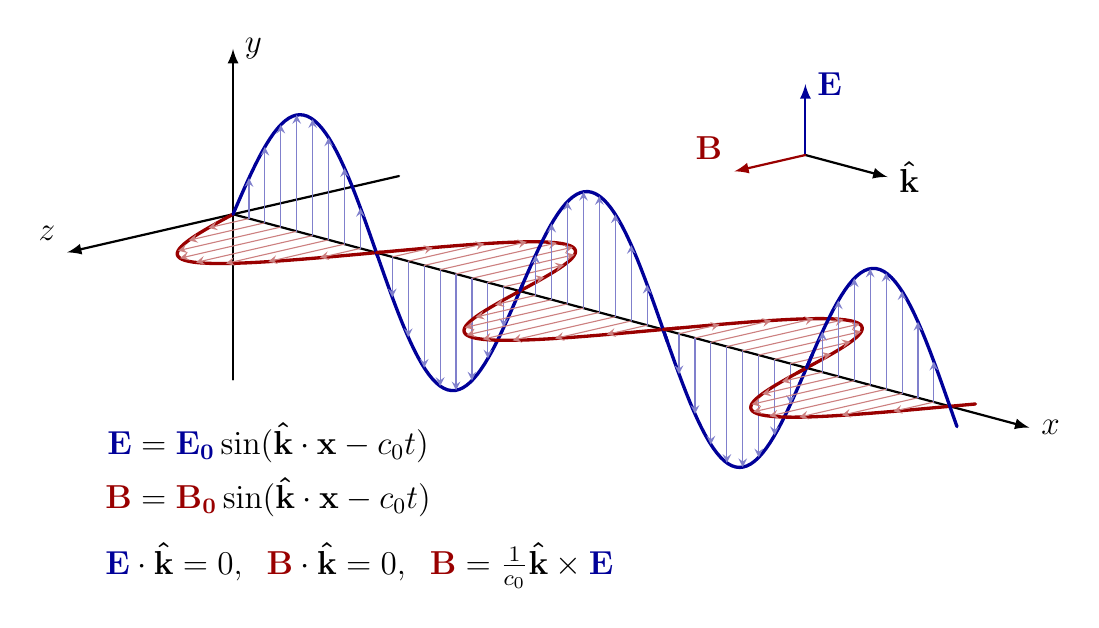
\begin{tikzpicture}[x=(-15:1.2), y=(90:1.0), z=(-150:1.0),
                    line cap=round, line join=round,
                    axis/.style={black, thick,->},
                    vector/.style={>=stealth,->}]
  \large
  \def\A{1.5}
  \def\nNodes{5} % use even number
  \def\nVectorsPerNode{8}
  \def\N{\nNodes*40}
  \def\xmax{\nNodes*pi/2*1.01}
  \pgfmathsetmacro\nVectors{(\nVectorsPerNode+1)*\nNodes}
 
  \def\vE{{\color{myblue}\mathbf{E}}}
  \def\vB{{\color{myred}\mathbf{B}}}
  \def\vk{\mathbf{\hat{k}}}
 
  \def\drawENode{ % draw E node and vectors with some offset
    \draw[myblue,very thick,variable=\t,domain=\iOffset*pi/2:(\iOffset+1)*pi/2*1.01,samples=40]
      plot (\t,{\A*sin(\t*360/pi)},0);
    \foreach \k [evaluate={\t=\k*pi/2/(\nVectorsPerNode+1);
                           \angle=\k*90/(\nVectorsPerNode+1);}]
                in {1,...,\nVectorsPerNode}{
      \draw[vector,myblue!50]  (\iOffset*pi/2+\t,0,0) -- ++(0,{\A*sin(2*\angle+\iOffset*180)},0);
    }
  }
  \def\drawBNode{ % draw B node and vectors with some offset
    \draw[myred,very thick,variable=\t,domain=\iOffset*pi/2:(\iOffset+1)*pi/2*1.01,samples=40]
      plot (\t,0,{\A*sin(\t*360/pi)});
    \foreach \k [evaluate={\t=\k*pi/2/(\nVectorsPerNode+1);
                           \angle=\k*90/(\nVectorsPerNode+1);}]
                in {1,...,\nVectorsPerNode}{
      \draw[vector,myred!50]  (\iOffset*pi/2+\t,0,0) -- ++(0,0,{\A*sin(2*\angle+\iOffset*180)});
    }
  }
 
  % main axes
  \draw[axis] (0,0,0) -- ++(\xmax*1.1,0,0) node[right] {$x$};
  \draw[axis] (0,-\A*1.4,0) -- (0,\A*1.4,0) node[right] {$y$};
  \draw[axis] (0,0,-\A*1.4) -- (0,0,\A*1.4) node[above left] {$z$};
 
  % small axes
  \def\xOffset{{(\nNodes-2)*pi/2}}
  \def\yOffset{\A*1.2}
  \def\zOffset{\A*1.2}
  \draw[axis,black] (\xOffset,\yOffset,-\zOffset) -- ++(\A*0.6,0,0) node[right,align=center] {$\mathbf{\hat{k}}$}; %\\propagation
  \draw[axis,myblue]  (\xOffset,\yOffset,-\zOffset) -- ++(0,\A*0.6,0) node[right] {$\mathbf{E}$};
  \draw[axis,myred]   (\xOffset,\yOffset,-\zOffset) -- ++(0,0,\A*0.6) node[above left] {$\mathbf{B}$};
 
  % equation
  \node[above right] at (\xOffset,-0.5*\yOffset,4*\zOffset)
    {$\begin{aligned}
      \vE &= {\color{myblue}\mathbf{E_0}}\sin(\vk\cdot\mathbf{x}-c_0t)\\
      \vB &= {\color{myred} \mathbf{B_0}}\sin(\vk\cdot\mathbf{x}-c_0t)\\
      \end{aligned}$};
  \node[below right] at (\xOffset,-0.5*\yOffset,4*\zOffset)
    {$\vE\cdot\vk = 0,\;\; \vB\cdot\vk = 0,\;\; \vB = \frac{1}{c_0}\vk\times\vE$};
 
  % draw (anti-)nodes
  \foreach \iNode [evaluate={\iOffset=\iNode-1;}] in {1,...,\nNodes}{
    \ifodd\iNode \drawBNode \drawENode % E overlaps B
    \else        \drawENode \drawBNode % B overlaps E
    \fi
  }
 
\end{tikzpicture}


\newpage

\begin{table}[!htbp] \centering 
  \caption{} 
  \label{} 
\begin{tabular}{@{\extracolsep{5pt}}lD{.}{.}{-3} D{.}{.}{-3} D{.}{.}{-3} D{.}{.}{-3} } 
\\[-1.8ex]\hline 
\hline \\[-1.8ex] 
 & \multicolumn{4}{c}{Linear Regression} \\ 
\cline{2-5} 
\\[-1.8ex] & \multicolumn{4}{c}{Year on Year GDP (in \%)} \\ 
\\[-1.8ex] & \multicolumn{1}{c}{(1)} & \multicolumn{1}{c}{(2)} & \multicolumn{1}{c}{(3)} & \multicolumn{1}{c}{(4)}\\ 
\hline \\[-1.8ex] 
 Constant & 3.434^{***} & 1.102^{***} & -0.920 & -1.403^{*} \\ 
  & (0.170) & (0.254) & (0.589) & (0.725) \\ 
  & & & & \\ 
 3 months lag of YoY GDP &  & 0.693^{***} & 0.575^{***} &  \\ 
  &  & (0.065) & (0.070) &  \\ 
  & & & & \\ 
 BSI & 14.867^{***} & 4.834^{***} & 9.064^{***} & 19.938^{***} \\ 
  & (1.351) & (1.367) & (1.717) & (1.373) \\ 
  & & & & \\ 
 Variance &  &  & 22.630^{***} & 45.301^{***} \\ 
  &  &  & (6.016) & (6.652) \\ 
  & & & & \\ 
\hline \\[-1.8ex] 
Observations & \multicolumn{1}{c}{124} & \multicolumn{1}{c}{123} & \multicolumn{1}{c}{123} & \multicolumn{1}{c}{124} \\ 
R$^{2}$ & \multicolumn{1}{c}{0.498} & \multicolumn{1}{c}{0.742} & \multicolumn{1}{c}{0.770} & \multicolumn{1}{c}{0.637} \\ 
Adjusted R$^{2}$ & \multicolumn{1}{c}{0.494} & \multicolumn{1}{c}{0.738} & \multicolumn{1}{c}{0.764} & \multicolumn{1}{c}{0.631} \\ 
Residual Std. Error & \multicolumn{1}{c}{1.174} & \multicolumn{1}{c}{0.848} & \multicolumn{1}{c}{0.805} & \multicolumn{1}{c}{1.002} \\ 
F Statistic & \multicolumn{1}{c}{121.091$^{***}$} & \multicolumn{1}{c}{172.776$^{***}$} & \multicolumn{1}{c}{132.525$^{***}$} & \multicolumn{1}{c}{106.248$^{***}$} \\ 
\hline 
\hline \\[-1.8ex] 
\textit{Note:}  & \multicolumn{4}{r}{$^{*}$p$<$0.1; $^{**}$p$<$0.05; $^{***}$p$<$0.01} \\ 
\end{tabular} 
\end{table} 


\newpage

\begin{tikzpicture}
\begin{axis}[
    domain=0:6*pi,
    samples=100,
    axis lines*=left, 
    axis line style={->},
    xtick={2.2, 4.5, 8.1}, ytick=\empty,
    xticklabels = {$Peak$, $Peak$, $Peak$},
    width=14cm, height=8cm,
    xlabel={time}, ylabel={GDP}
]       
\addplot[mark=none, dashed] coordinates {(2.2, -1) (2.2, 4)};
\addplot[mark=none, dashed] coordinates {(4.5, -1) (4.5, 1)}; 
\addplot[mark=none, dashed] coordinates {(8.1, -1) (8.1, 12)}; %\addplot [thick, gray] {x};
\addplot [thick, black] {x + 4*sin(deg(x)) * sin(deg(x/6))^0.5}
%    node [pos=0.1, anchor=south] {Peak}
    node [pos=0.3, anchor=south, sloped] {Expansion}
    node [pos=0.49, anchor=south, sloped] {Recession}
% Add line to show end of and ... peak and ... line
;
\end{axis}
\end{tikzpicture}




\end{document}